\newcommand{\texMacro}[2]{\texttt{\textbackslash{#1}\{#2\}}}
% \section{General LaTeX tips}\label{sec:latex_tips}
% Some tips were given in \Cref{sec:intro}, and this section will elaborate with some more concrete examples.
\section{Optimal Control of Pitch/Travel without Feedback}\label{sec:latex_tips}

\subsection{Continuous State Space Form}
% Write the model on continuous time state space form
First we must formulate the model (\ref{eq:model}) in a continuous state-space form. Elevation is neglected here.

The equation for elevation (\ref{eq:model_se_elev}) is completely removed from the model (\ref{eq:model}) and we are left with the following set of equations.

\begin{subequations}
	\begin{align}
		\ddot{p} = - K_1K_{pd}\dot{p} - K_1K_{pp}p + K_1K_{pp}p_c \\
		\dot{\lambda} = r \\
		\dot{r} = -K_2p
	\end{align}
\end{subequations}

Since $ \vec{x} = [\lambda\ r\ p\ \dot{p}]^T $, and $ u = p_c $ we can formulate $\ddot{p}$ as a vector product.

\begin{equation}
	\ddot{p} = [0\ 0\ -K_1K_{pp}\ -K_1K_{pd}]^T \vec{x} + [K_1K_{pp}]^T u
\end{equation}

We can get the change in $ p $ as:

\begin{equation}
\dot{p} = [0\ 0\ 0\ 1]^T \vec{x} + [0]^T u
\end{equation}

Likewise for $ r $:
\begin{equation}
	\dot{r} = [0\ 0\ -K_2\ 0]^T \vec{x} + [0]^T u
\end{equation}
and finally for $\lambda$:
\begin{equation}
	\dot{\lambda} = [0\ 1\ 0\ 0]^T \vec{x} + [0]^T u
\end{equation}

Using the formulas that were given we were able to construct a state-space model of form in (\ref{eq:state-space}).
\begin{equation}\label{eq:state-space}
	\vec{\dot{x}} = A_c \vec{x} + \vec{B_c} u
\end{equation}

\begin{subequations}
\begin{align}
\alpha_1 = K_1K_{pp} \\
\alpha_2 = K_1K_{pd} \\
A_c =
\begin{bmatrix}
    0 & 1 & 0 & 0 \\
    0 & 0 & -K_2 & 0 \\
    0 & 0 & 0 & 1 \\
    0 & 0 & -\alpha_1 & - \alpha_2
\end{bmatrix}
\label{eq:initial_state}
\end{align}
\end{subequations}

\begin{equation}
B_c =
\begin{bmatrix}
	0 \\
	0 \\
	0 \\
	\alpha_1
\end{bmatrix}
\end{equation}

% What are we modeling here? Is it just the helicopter? Discuss what the model includes, and how it relates to Figure 7.
The aforementioned model various states of the helicopter; including pitch, distance traveled, travel speed, and the input and its effects on these variables. Additionally we make the  simplifying assumptions that the pitch angle is small, and that there is no friction or air resistance acting on the helicopter resisting the direction of travel. Figure (APPENDIX FIGURE 7) contains the precomputed $u*$ which are fed into the system.

\subsection{Forward Euler Discretization}
% Discretize the model using the forward Euler method and write the resulting model on discrete time state space form

Using Euler's time discretization on the system's standard form we will get the following expression:

\begin{equation}
	x_{k+1} = Ax_k + Bu_k
\end{equation}
First we discretize the derivative vector
\begin{subequations}
\begin{align}
\vec{\dot{x}} = \lim_{h\rightarrow 0} \frac{\vec{x}_{k+1}-\vec{x}_{k}}{h} \\
\Rightarrow \vec{\dot{x}} = \lim_{h\rightarrow 0} \frac{\vec{x}_{k+1}-\vec{x}_{k}}{h} = \mathbf{A_c} \vec{x}_k + \vec{B_c} u_k
\end{align}
\end{subequations}
We ignore the limit, it's implicit for $ h $.
\begin{equation}
\Rightarrow \vec{x}_{k+1} = \vec{x}_{k} + h(\mathbf{A_c} \vec{x}_k + \vec{B_c} u_k)
\end{equation}
Now $ \vec{x}_k $ can be algebraically merged into a matrix.
\begin{subequations}
\begin{align}
\Rightarrow \vec{x}_{k+1} = h{A_c} \vec{x}_k + \vec{x}_{k} + h\vec{B_c} u_k \\
\Rightarrow \vec{x}_{k+1} = (h{A_c} \mathbf{I} + \mathbf{I})\vec{x}_k + h\vec{B_c} u_k
\end{align}
\end{subequations}
This is the same as adding $ 1 $ to each diagonal in $ h\mathbf{A_c} $. We rename it ($hA_c\mathbf{I} + \mathbf{I}$) to $ {A}$ and ($h\vec{B_c}$) to $B$.
\begin{equation} \label{mat:eq}
\Rightarrow \vec{x}_{k+1} = \mathbf{A} \vec{x}_k + \vec{B} u_k
\end{equation}
Where
\begin{equation}
\mathbf{A} = h\mathbf{A_c} + \mathbf{I}
\end{equation}
\begin{equation}
\vec{B} = h\vec{B_c}
\end{equation}

\subsection{Calculate an Optimal Trajectory}
%  Calculate an optimal trajectory for moving the helicopter from x 0 = λ 0 0 0 0 to x f = λ f 0 0 0 when the elevation angle is assumed to be constant. Use λ 0 = π and λ f = 0. Also implement the constraint 30π |p k | ≤ , k ∈ {1, . . . , N } [14] 180 Since the manipulated variable p c in this case is the setpoint for the p controller, the constraint should also be implemented for the manipu- lated variable. We want to minimize the cost function N [λ i − λ f ] 2 + qp 2 ci , φ = q ≥ 0 [15] i=1 Solve the optimization problem using the MATLAB function quad- prog. Try using the values 0.1, 1, and 10 as weights q. Plot the manipulated variable and the output. Comment the results with re- spect to the different weights chosen. Remember that some useful files are posted on Blackboard. Use a sampling time of 0.25 s and N = 100.  15Furthermore, discuss the objective function [15], in particular the term [λ i − λ f ] 2 . For instance, could any unwanted effects arise from steer- ing the helicopter to λ = λ f with this objective function?
We encode the equality constraint using \ref{mat:eq}, this gives us a constraint where we have a matrix of the form
\begin{equation}
A_{eq} =
\begin{bmatrix}
    I      & 0  & 0 & 0 & \hdots & 0      & 0  & -B & 0  & 0  & \hdots & 0\\
    -A     & I  & 0 & 0 &        & 0      & 0  & 0  & -B & 0  &        & 0\\
    0      & -A & I & 0 &        & 0      & 0  & 0  & 0  & -B &        & 0\\
    \vdots &    &   &   & \ddots & \vdots & 0  &    &    &    & \ddots & \vdots\\
    0      & 0  & 0 & 0 & \hdots & -A     & I  & 0  & 0  & 0  & \hdots & -B\\
\end{bmatrix}
\end{equation}

With the constraint
\begin{equation}
\mathbf{A}_{eq}^{[400x500]} \vec{x} = \vec{B}_{eq}
\end{equation}
Where
\begin{equation}
\vec{B}_{eq}[t] = \vec{0}\ \forall t > 1
\end{equation}
\begin{equation}
\vec{B}_{eq}[1] = Ax_0
\end{equation}

The following plots convey our theoretical and practical results:

The graphs with the circles are theoretical and the one with only blue line graphs are practical. There are significant differences between these.

One can observe that setting $ q = 0.1 $ does not particularly affect travel rate in practice, but setting $ q = 10 $ affects travel rate significantly.

The objective function collapses into just

$$ \sum_{i=1}^N \lambda_i^2 + qp_{ci}^2 $$

when $ \lambda_f = 0 $. This term is not scaled (except for unit scaling) such that we can fully control the objective function by exploiting $ q $. An unwanted effect could be overshoot, since a high q is more keen on keep $ p_{ci} $.

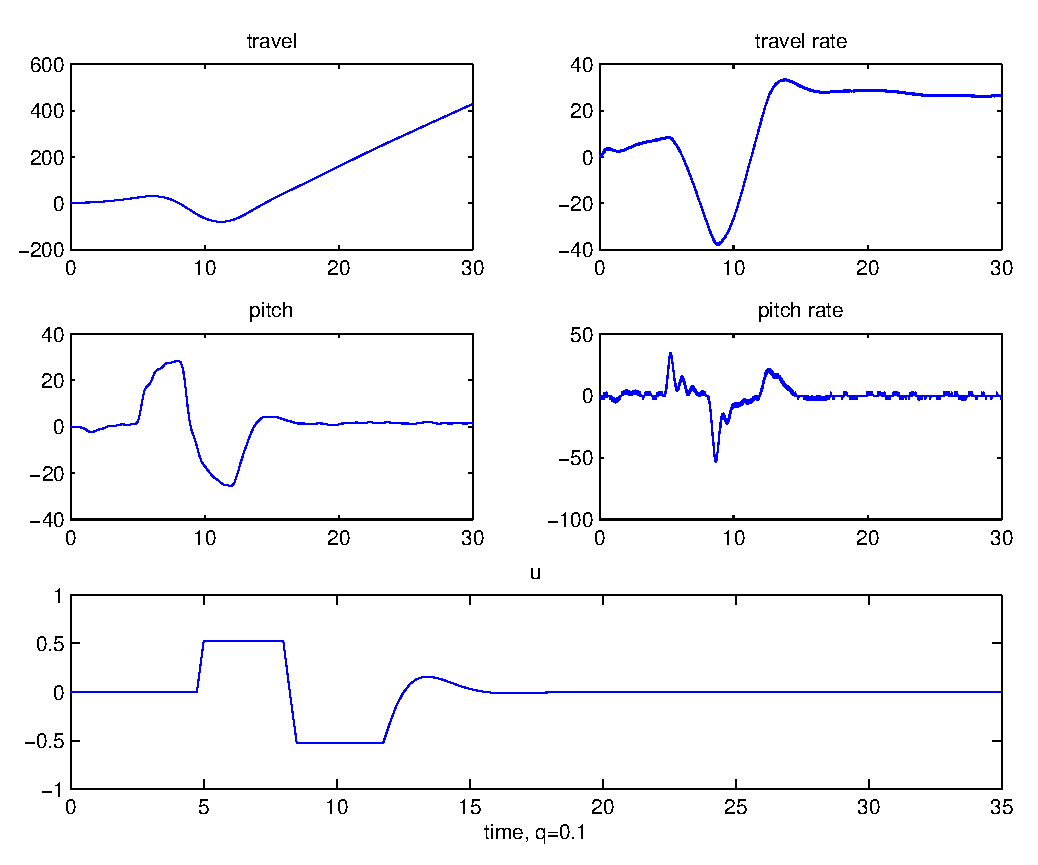
\includegraphics{{figures/10.2.3.q_0.1}.eps}
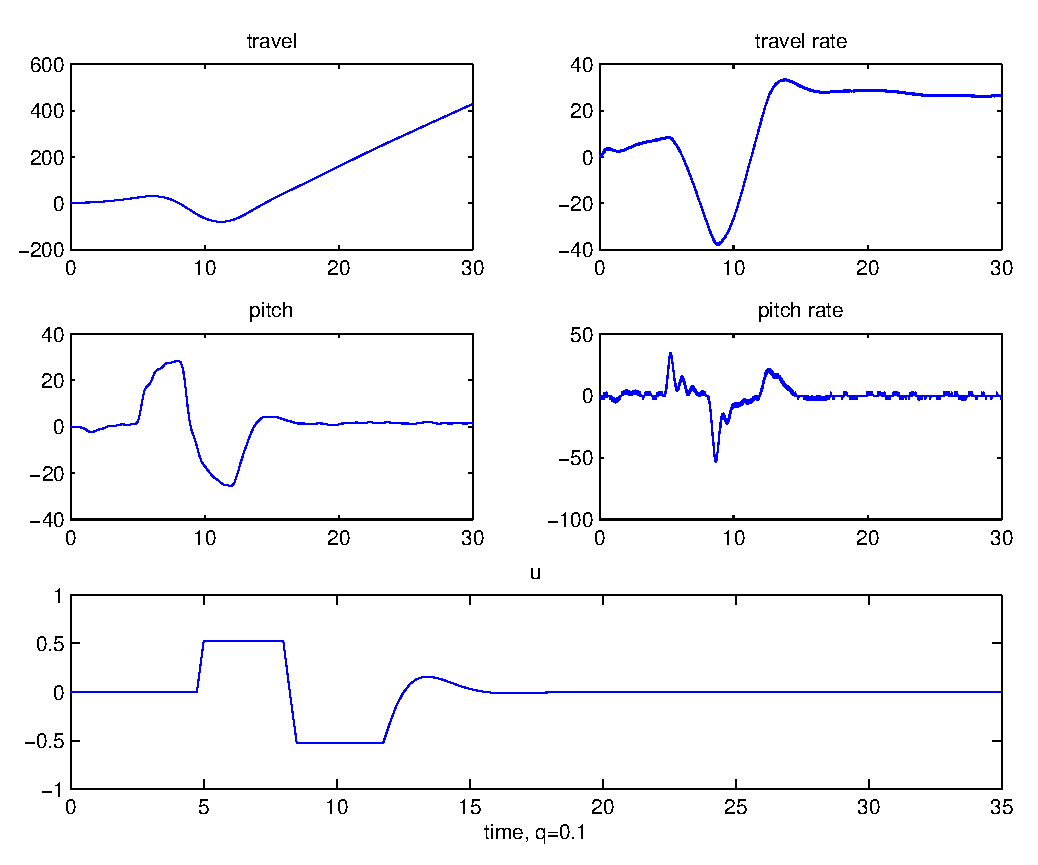
\includegraphics{{figures/10.2.3.q_0.1.theory}.eps}

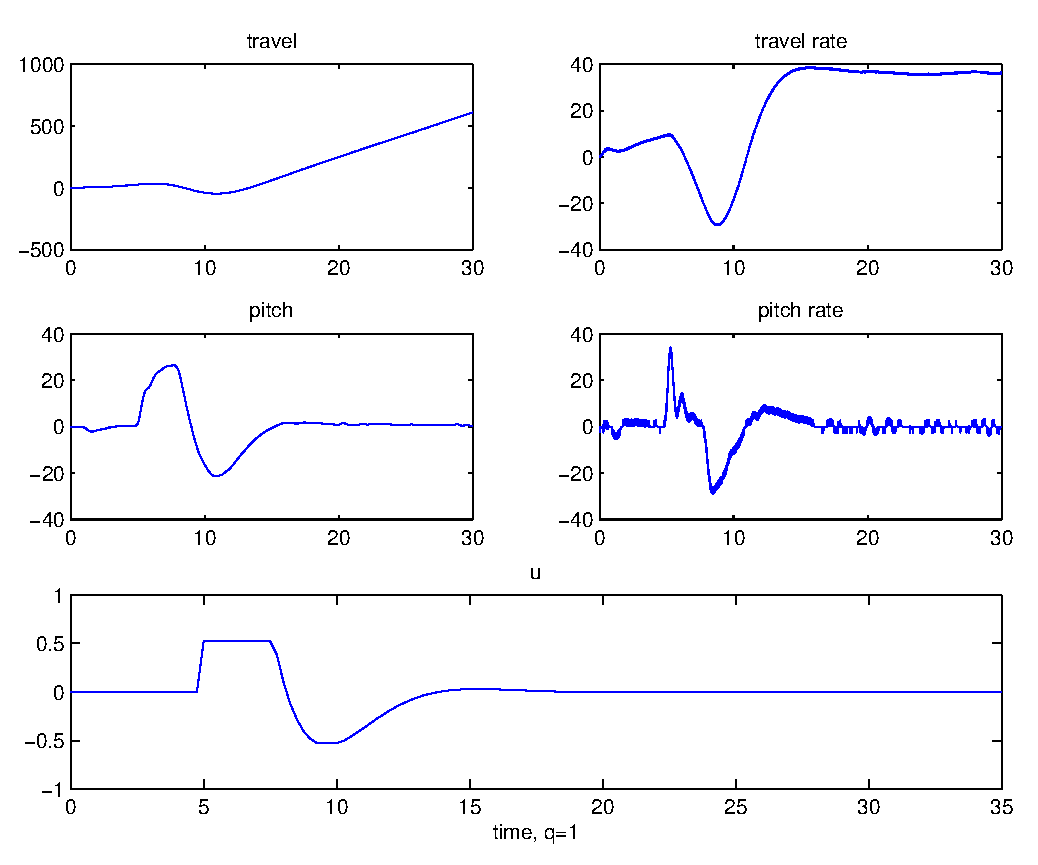
\includegraphics{{figures/10.2.3.q_1}.eps}
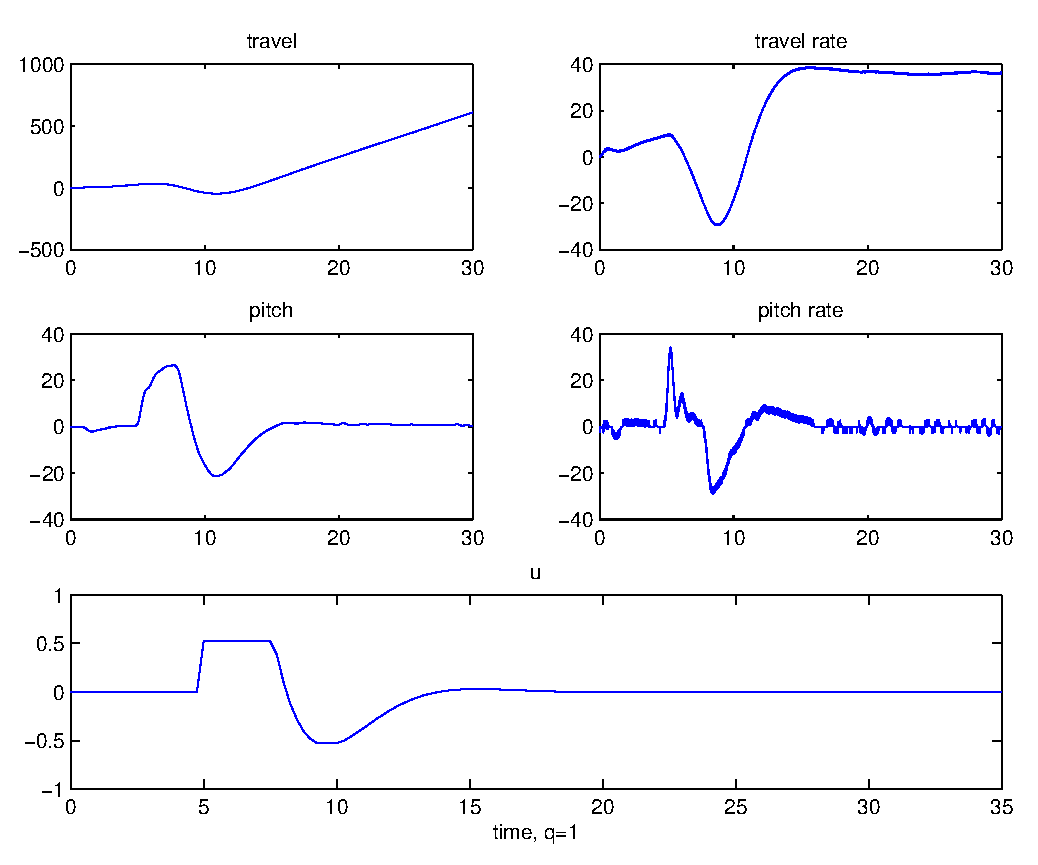
\includegraphics{{figures/10.2.3.q_1.theory}.eps}


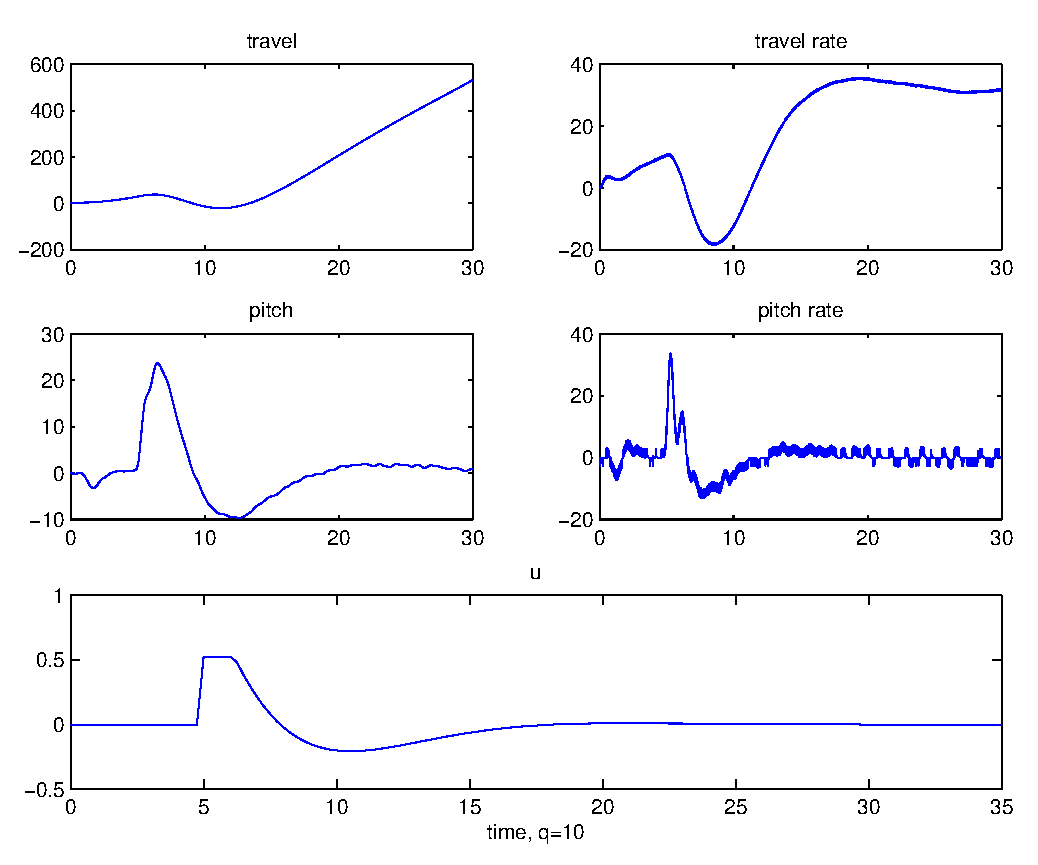
\includegraphics{{figures/10.2.3.q_10}.eps}
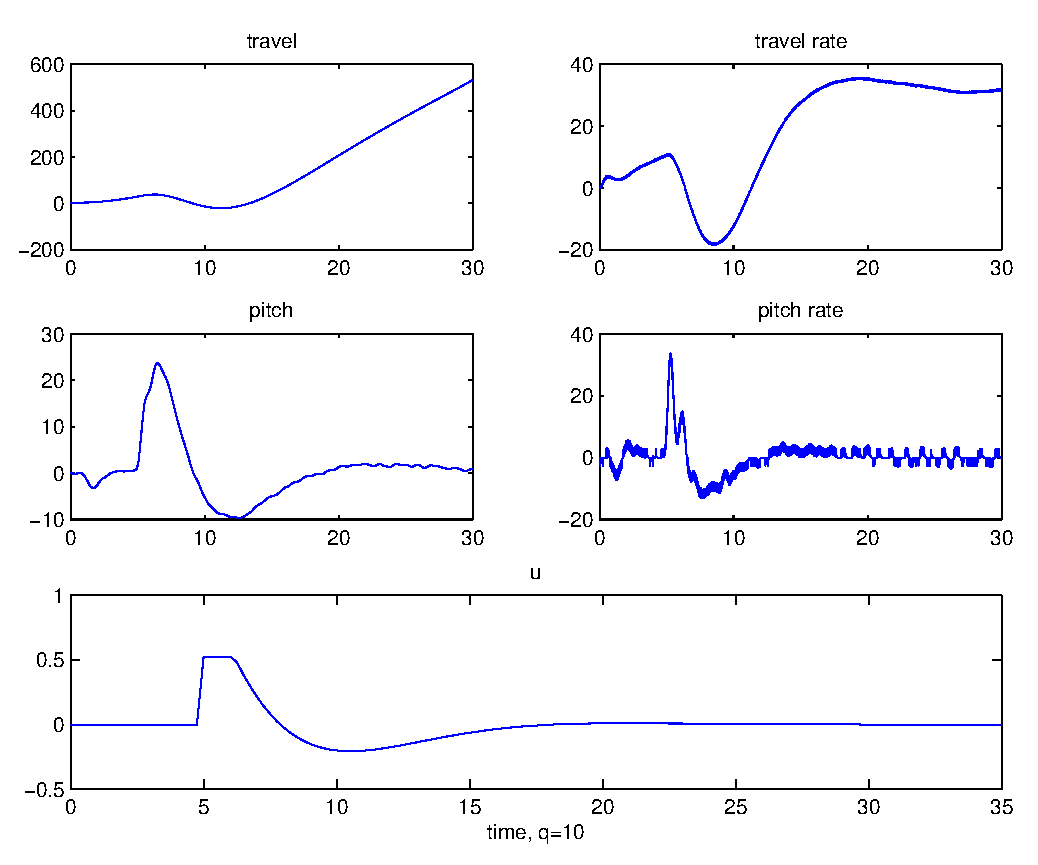
\includegraphics{{figures/10.2.3.q_10.theory}.eps}

\subsection{Offset}
% The specific implementation of the QP algorithm used here can only weight deviations from origin [λ f = 0]. The position sensors on the helicopter are relative, which means that the position is reset to zero each time the helicopter is started. To get the helicopter to start in x 0 you have to add a suitable value to the measurement. For example, you can subtract 30 ◦ from the elevation measurement to get the helicopter to fly at a reasonable height when e c = 0 [this is done in the given file]. Implement the input sequence generated in c] with q = 1.  The optimization in c] gives the manipulated variable u. It may be a good idea to add some zeros at the beginning of the input vector, so that the helicopter has time to stabilize in x 0 before the calculated sequence is implemented. Also, adding zeros at the end of the vector is recommended to keep the helicopter stable after the input sequence is over. Add enough zeros to keep the helicopter stable for at least 5 s before and after the optimal input sequence is implemented. The easiest way to transfer the input sequence to Simulink is to use a “From Workspace” block [which can be found under “Sources” in the Library Browser]. This block imports two vectors, a vector u which is connected to the output and a time vector t which determines when the different elements of u should be transfered to the output.  Does the helicopter end in the desired point x f ? What causes the observed deviation?

We implemented this optimal control sequence on the test helicopters and observed noticeable deviation from the desired final position. This is due to lack of feedback to account for physical disturbances, modeling inconsistencies and linearizion errors.

We see from the following figure that the travel is reversed by the input variable.

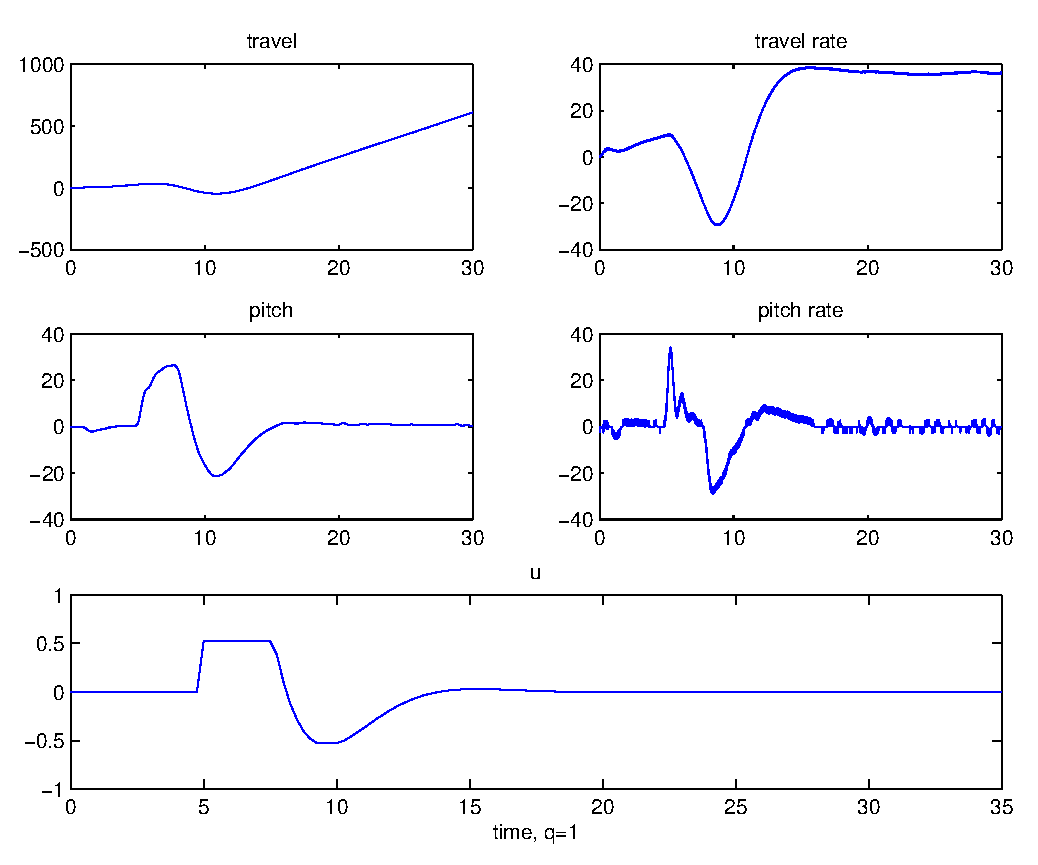
\includegraphics{{figures/10.2.3.q_1}.eps}

\section{Optimal Control of Pitch/Travel with Feedback (LQ)}

\subsection{LQ Control}
% In MATLAB you can use the function dlqr to calculate the optimal K matrix. Q and R indicates how much you want to penalize deviation in the states, and how much you want to penalize use of the manipulated variable. Use diagonal matrices for Q and R. A diagonal matrix is easily made in MATLAB using the function diag.
Feedback in the optimal controller:

\lstinputlisting[language=Matlab]{compute_lq.m}

\subsection{Simulink Feedback}
% Implement the feedback on the helicopter and run the helicopter. This is done in Simulink using the following blocks Mux, Demux, Matrix 17Multiplication, Sum, and “From Workspace”. Notice that the “From Workspace” block can import several values [a vector], meaning only one block is required for x.
Please see the model (REFERENCE HERE).

\subsection{MPC Controller}
% An alternative strategy would be to use an MPC controller. How would you realize this controller?
We would realize the MPC controller by creating a matlab function block in the simulink diagram that uses the current state as an initial state in the horizon. After solving the horizon for $u$, we supply the first element of $u$ to as input.

% Discuss advantages and disadvantages with and MPC controller compared to the controller you have implemented.
The MPC controller may be significantly more expensive. The LQR is much simpler in that it takes one big computation on that generates a multiplication matrix which does not need to be recomputed. In essence the MPC controller needs to solve this at every time step which may be more costly to run. The LQR controller is also simpler in its design.

% Also, think about how the structure in Figure 8 would look if you used MPC.

\section{Optimal Control of Pitch/Travel and Elevation with and without Feedback}
\subsection{Continuous State Space Form}
% Write the system on continuous state space form with the two extra states e and e.  ̇ Use x = λ r p p  ̇ e e  ̇ and u = p c e c
Given the following equation for elevation:
\begin{equation}\label{eq:elevation}
\ddot{e} = -K_3K_{ed}\dot{e} - K_3K_{ep}e +K_3K_{ep}e_c
\end{equation}

Using (\ref{eq:elevation}) and converting it into a state-space model:
$$
\begin{bmatrix}
\dot{e} \\
\ddot{e}
\end{bmatrix} = \begin{bmatrix}
0 & 1 \\
-K_3K_{ep} & -K_3K_{ed}
\end{bmatrix}\begin{bmatrix}
e \\
\dot{e}
\end{bmatrix}
+\begin{bmatrix}
0 \\
K_3K_{ep}
\end{bmatrix}e_c
$$

Merging this with (\ref{eq:initial_state}) yields

\begin{equation}
\bar{A}_c =
\begin{bmatrix}
    0 & 1 & 0 & 0 & 0 & 0 \\
    0 & 0 & -K_2 & 0 & 0 & 0 \\
    0 & 0 & 0 & 1 & 0 & 0 \\
    0 & 0 & -\alpha_1 & - \alpha_2 & 0 & 0 \\
    0 & 0 & 0 & 0 & 0 & 1 \\
    0 & 0 & 0 & 0 & -K_3K_{ep} & -K_3K_{ed}
\end{bmatrix}
\end{equation}

\begin{equation}
\bar{B}_c =
\begin{bmatrix}
    0 & 0\\
    0 & 0 \\
    0 & 0 \\
    \alpha_1 & 0 \\
    0 & 0 \\
    0 & K_3K_{ep}
\end{bmatrix}
\end{equation}

Completing the system by forming the expression

\begin{equation}
\dot{x} = A_c\ x + B_c\ x
\end{equation}

\subsection{Forward Euler Discretization}
% Discretize the model using the forward Euler method and write the resulting model on discrete state space form.

Using the same technique as previously utilized:

$$ \dot{x} = \bar{A}_c x + \bar{B}_c u $$
$$ \Rightarrow \frac{x_{t+1} - x_t}{T} = \bar{A}_c x_t + \bar{B}_c u_t $$
$$ \Rightarrow x_{t+1} = x_t + T\bar{A}_c x_t + T\bar{B}_c u_t $$
$$ \Rightarrow x_{t+1} = (I + T\bar{A}_c) x_t + T\bar{B}_c u_t $$

Yielding new matrices for the discrete case:

\begin{equation}
\bar{A} =
\begin{bmatrix}
    1 & T & 0 & 0 & 0 & 0 \\
    0 & 1 & -TK_2 & 0 & 0 & 0 \\
    0 & 0 & 1 & T & 0 & 0 \\
    0 & 0 & -T\alpha_1 & 1-T\alpha_2 & 0 & 0 \\
    0 & 0 & 0 & 0 & 1 & T \\
    0 & 0 & 0 & 0 & -TK_3K_{ep} & 1-TK_3K_{ed}
\end{bmatrix}
\end{equation}

\begin{equation}
\bar{B} =
\begin{bmatrix}
    0 & 0 \\
    0 & 0 \\
    0 & 0 \\
    T\alpha_1 & 0 \\
    0 & 0 \\
    0 & TK_3K_{ep}
\end{bmatrix}
\end{equation}

Where $T$ is the time step.

\subsection{SQP Algorithm}
Nothing here

\subsection{Optimal Input on Helicopter}
% Implement the optimal input sequence on the helicopter. Introduce feedback in the same way as in exercise 3. Compare the performance with and without feedback.
We'll need some GRAPHS here >:)

\subsection{Decoupled States}
% Notice that the first 4 states in the model are completely decoupled from the last 2. How does this fit with reality? What effect does this have on the calculated optimal trajectory? Suggest [but do not implement] a solution to improve this.

\subsection{Adding More Constraints}
% Optional exercise: Try adding more constraints on the states. These ̇may be constraints on maximal allowed speed e  ̇ and λ.

% \subsection{Tables}
% If you want, you can use the source for \Cref{tab:parameters} to see how a (floating) table is made.

% \begin{table}[tbp]
% 	\centering
% 	\caption{Parameters and values.}
% 	\begin{tabular}{llll}
% 		\toprule
% 		Symbol & Parameter & Value & Unit \\
% 		\midrule
% 		$l_a$ & Distance from elevation axis to helicopter body & $0.63$ & \meter\\
% 		$l_h$ & Distance from pitch axis to motor & $0.18$ & \meter\\
% 		$K_f$ & Force constant motor & $0.25$ & \newton\per\volt\\
% 		$J_e$ & Moment of inertia for elevation & $0.83$ & \kilogram\usk\meter\squared\\
% 		$J_t$ & Moment of inertia for travel & $0.83$ & \kilogram\usk\meter\squared\\
% 		$J_p$ & Moment of inertia for pitch & $0.034$ & \kilogram\usk\meter\squared\\
% 		$m_h$ & Mass of helicopter & $1.05$ & \kilogram\\
% 		$m_w$ & Balance weight & $1.87$ & \kilogram\\
% 		$m_g$ & Effective mass of the helicopter & $0.05$ & \kilogram\\
% 		$K_p$ & Force to lift the helicopter from the ground & $0.49$ & \newton\\
% 		\bottomrule
% 	\end{tabular}
% \label{tab:parameters}
% \end{table}

% There is also a lot of useful software to manage your references. Some popular examples include JabRef (\url{http://www.jabref.org/}), Mendeley (\url{https://www.mendeley.com/}) and EndNote. JabRef is perhaps the simplest of these three, and stores all information in a \texttt{.bib} file that you can directly use in your Latex document. Both Mendeley and EndNote can export references as BibTeX.
